% PP-Article.tex for AEA last revised 22 June 2011
\documentclass[twocolumn, a4paper]{article}

%%%%%% NOTE FROM OVERLEAF: The mathtime package is no longer publicly available nor distributed. We recommend using a different font package e.g. mathptmx if you'd like to use a Times font.
\usepackage{mathptmx}
\usepackage{amsmath}
\usepackage[dutch]{babel}
\usepackage{subcaption}
\usepackage[width=.8\textwidth]{caption}
\usepackage{float}
\usepackage[utf8]{inputenc}
\usepackage{booktabs}
\usepackage{multicol}
\usepackage{longtable}
\usepackage{minted}
% If you have trouble with the mathtime package please see our technical support 
% document at: http://www.aeaweb.org/templates/technical_support.pdf
% You may remove the mathtime package if you can't get it working but your page
% count may be inaccurate as a result.
% \usepackage[cmbold]{mathtime}
\usepackage{xargs}                      % Use more than one optional parameter in a new commands 
\usepackage[pdftex,dvipsnames]{xcolor}  % Coloured text etc.
% 
\usepackage{pdfpages}
\usepackage[colorinlistoftodos,prependcaption,textsize=tiny]{todonotes}
\newcommandx{\unsure}[2][1=]{\todo[linecolor=red,backgroundcolor=red!25,bordercolor=red,#1]{#2}}
\setlength{\marginparwidth}{2cm}
% Note: you may use either harvard or natbib (but not both) to provide a wider
% variety of citation commands than latex supports natively. See below.

% Uncomment the next line to use the natbib package with bibtex 
%\usepackage{natbib}
\usepackage{titlesec}

\titlespacing*\section{0pt}{12pt plus 4pt minus 2pt}{0pt plus 2pt minus 2pt}
\titlespacing*\subsection{0pt}{12pt plus 4pt minus 2pt}{0pt plus 2pt minus 2pt}
\titlespacing*\subsubsection{0pt}{12pt plus 4pt minus 2pt}{0pt plus 2pt minus 2pt}



% Uncomment the next line to use the harvard package with bibtex
%\usepackage[abbr]{harvard}

% This command determines the leading (vertical space between lines) in draft mode
% with 1.5 corresponding to "double" spacing.
\begin{document}

\title{Geavanceerde computerarchitectuur: Labo 02' \\ 
\large{Uitbreiding: OpenCL}}
\author{\textsc{Anton Danneels en Pieter Delobelle}}
\date{}
\maketitle

\section{Inleiding}


\section{Analyse}

\subsection{OpenCL}
OpenCL is---net als CUDA---een framework en platform om berekeningen te kunnen uitvoeren op GPU's, maar biedt ook meer flexibiliteit door ook CPU's en andere \emph{hardware accelerators} te ondersteunen. Daarnaast is OpenCL ook een open standaard die door verschillende fabrikanten wordt gevolgd, in tegenstelling tot CUDA van NVIDEA.

Omdat OpenCL meerdere \emph{vendors} en systemen ondersteunt, is er een hiërarchische organisatie om verschillende apparaten aan te sturen. Ten eerste zijn gelijkaardige systemen gegroepeerd per \emph{platform}. OpenCL-kernels worden gecompileerd voor een bepaald platform. 

Ten tweede worden platformen opgedeeld in \emph{devices}. Dit is iedere CPU, GPU of andere \emph{hardware accelerator} onder een bepaald platform. Logischerwijs heeft ieder apparaat enkele eigenschappen, zoals kloksnelheid en het aantal \emph{work units}, die een invloed hebben op de resulterende uitvoersnelheid voor een bepaalde kernel.

\begin{minted}{c}
    const int2 pos = {
            get_global_id(0), 
            get_global_id(1)
        };
    \end{minted}
    \label{c:index}

Iedere OpenCL-kernel wordt uitgevoerd door één of meerdere \emph{work items}, wat equivalent is aan een CUDA-thread. Alle items krijgen enkele indices toegewezen: een globale index, een index binnen de work unit (local id) en de index van de work unit. Deze items worden dus gegroepeerd in blokken, die conceptueel overeenkomen met de \emph{wraps} uit CUDA. 

Omdat OpenCL echter ook op CPU's draait, is het kiezen van een optimale \emph{local work size} echter complexer. Hiervoor biedt OpenCL de optie om dit op NULL te laten, waardoor automatisch de beste grootte gekozen wordt.

\subsection{Kleurenruimte en kleurendiepte}
Verschillende operaties werken intern met een kleurendiepte die groter is dan de standaard diepte waarin een afbeelding wordt ingelezen (8 bits per component). Dit is problematisch voor operaties zoals vervagen, aangezien convoluties hier voor resultaten kunnen zorgen die groter zijn wat kan weergegeven worden in een getal van 8 bits (256). Een optie is hiervoor om grotere representaties te gebruiken, maar dit stelt het probleem enkel uit. Hierom is gekozen om intern te werken met een zwevendekommagetal (\emph{double}) Pas finaal worden alle waarden gecast naar een 8-bits getal.

Een tweede kwestie is in welke kleurruimte operaties uitgevoerd worden. Standaard worden bestanden ingelezen in RGB of RGBA indien er een \emph{alpha}-kanaal aanwezig is, maar andere kleurruimtes kunnen voor bepaalde operaties voordeliger zijn.

\begin{itemize}
    \item \textbf{RGB}: populair systeem dat kleuren encodeerd in 3 componenten, rood, groen en blauw. In het geval van RGB24 zijn er 16 miljoen kleuren mogelijk, maar voor recente ontwikkelingen omtrent \emph{high dynamic range} (HDR) is dit niet altijd meer toereikend. De meeste afbeeldingen zijn hierin echter zonder problemen te encoderen. 

    Bepaalde bewerkingen, zoals het aanpassen van saturatie, zijn echter zeer complex in RGB. 

    Daarnaast is het ook mogelijk om de RBG-ruimte niet-lineair te encoderen. Hierdoor kunnen bijvoorbeeld meer discrete zwartwaarden onderscheiden worden. Hiervoor wordt een parameter $\gamma$ geïntroduceerd.
    
    \item \textbf{HSL}: dit systeem encodeert de tint (\emph{hue}), saturatie en helderheid (\emph{lightness}) van een pixel. Het spreekt voor zich dat het aanpassen van deze componenten hierin zeer eenvoudig is. De tint kan voorgesteld worden in een kleurenwiel, wat dit systeem ook geschikt maakt voor kleureninput van gebruikers. Kleuren kunnen echter wel afwijken door interpolaties, wat het minder geschikt maakt voor bepaalde applicaties.

    \item \textbf{HSI}: Variant op HSL, maar met een intensiteit-parameter in plaats van de helderheid.  
    \item \textbf{CMYK}: additief kleurensysteem voor drukwerk, voor digitale verwerking biedt dit geen voordelen. 
    \item \textbf{CIE XYZ}: systeem gebaseerd op perceptie. Er is één helderheidscomponent (Y) en twee kleurencomponenten (X en Z). Dit systeem is zeer bruikbaar voor het mixen van kleuren.
    \item \textbf{CIElab}: Een tweede systeem met twee kleurencomponenten en een helderheidscomponent. Hier worden kleuren geëncodeerd als \emph{Luminance} en een combinatie van rood-groen en blauw-geel. Het is minder bruikbaar voor kleurtransformaties, maar is uniform (in tegenstelling to gequantiseerde modellen zoals RGB).
\end{itemize}

Voor de meeste operaties is een RBG-ruimte dus prima te doen, waarbij eventueel kan overgeschakeld worden naar CIE XYZ als intermediaire voorstelling mocht het mixen van kleuren gewenst zijn. 

\subsection{Gaussiaans vervagen}
Om OpenCL uit te testen werd een \textit{mask} toegepast op een afbeelding. Dit mask combineert pixels rondom een gekozen doelpixel, waarbij elke pixel een bepaald gewicht krijgt. E\'en van deze masks is de Gaussiaanse. Hierbij krijgen de pixels een gewicht gebaseerd op hun afstand tot het doelwit. De gewichten volgen zo een Gaussiaanse functie.

\subsection{Witpuntsverschuiving}
Het verschuiven van een witpunt van een afbeelding \todo{..}

\subsection{Qt}
Qt is een \emph{cross-platform} raamwerk voor gebruikersinterfaces te ontwikkelen, waarbij de achterliggende code in C++ geschreven kan worden. Het raamwerk volgt een object-geörienteerde strategie, door iedere GUI-element te modelleren als een object (QWidget) met hiërarchische overerving voor verschillende types van elementen, zoals knoppen (QButton).


\section{Oplossing}

\subsection{Pipeline}
Voor een foto verwerkt kan worden door een kernel moet eerst de OpenCL omgeving geconfigureerd worden. Dit bestaat uit de volgende stappen:

\begin{enumerate}
    \item Platforms en devices opvragen 
    \item Context aanmaken
    \item Programma compileren
    \item Command queue aanmaken
    \item Kernels configureren
\end{enumerate}
Pas indien dit gebeurd is, kan kernel op de command queue gezet worden zodat deze uitgevoerd kan worden. Om de resultaten uit te lezen wordt er gewacht op de command queue en vervolgens kan een leesopdracht gegeven worden aan de command queue. 

Om grotere hoeveelheden data naar de kernels te uploaden, wordt gebruik gemaakt van buffer objecten. Deze specificeren hoe de data er uit ziet en hoe groot deze is. In deze applicatie worden buffers gebruikt om de afbeeldingen en een kopie van de afbeelding door te sturen naar de kernel, samen met een mask.

\subsection{Apparaatselectie}
Pieter zijn QT code expanding-brain-4

\section{Evaluatie}

\subsection{Invloed van local work size}
Zoals eerder vermeld, hebben verschillende devices een verschillende hardwareconfiguratie. Hierdoor zijn bepaalde dimensies langzamer---aangezien de hardware niet ideaal gebruikt wordt---of zelfs niet mogelijk. Ieder device kan zijn eigen maxima rapporteren, wat voor een CPU veelal één is.

Voor een GPU (Device: AMD Radeon Pro 555 Compute Engine) is een meting uitgevoerd over alle combinaties van 1x1 tot 128x128. Hiervoor is een afbeelding van 1024x1024 van een zebra gekozen, met vier kleurencomponenten (RGBA). Per dimensie zijn er 5 metingen uitgevoerd. Hier resultaat is grafisch te zien in Figuur~\ref{fig:output-all}. De data staat ook op Github.

\begin{figure}
    \centering
    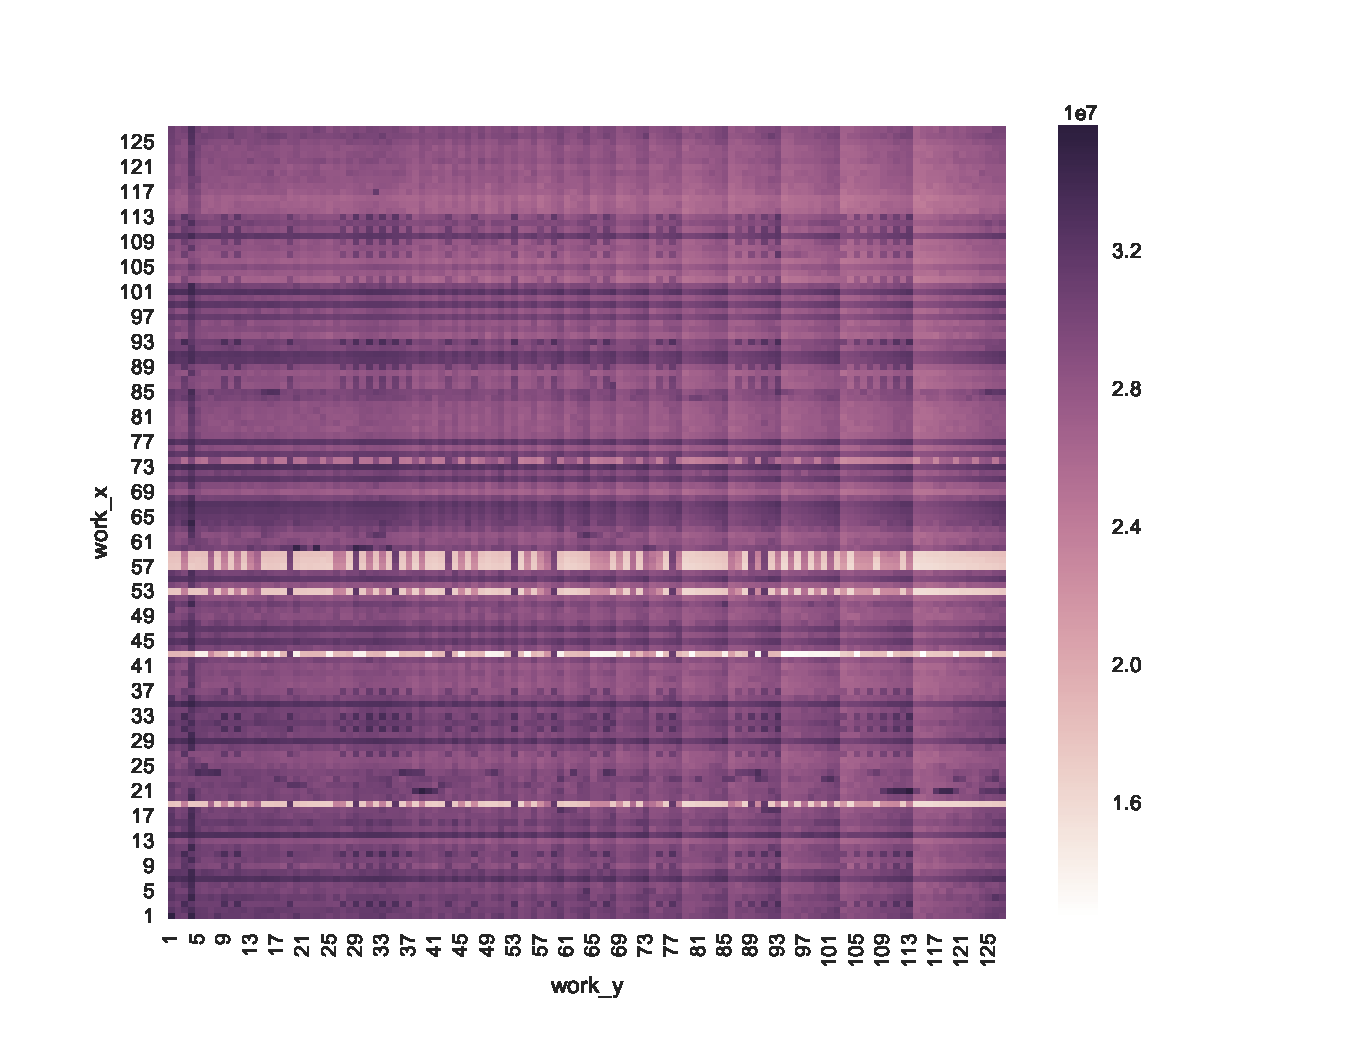
\includegraphics[width=0.55\textwidth]{data/output_all}
    \caption{Invloed van \emph{work size} op uitvoertijd (in ns).}\label{fig:output-all}
\end{figure}

\subsection{Vergelijking tussen devices}

\begin{table*}[]
    \centering
    \caption{Vergelijking tussen die OpenCL-devices op eenzelfde systeem.}
    \label{table:measurements}
    \begin{tabular}{@{}llrrr@{}}
        \toprule
        Abeelding & Formaat (w, h, comp) & Intel i7-7700HQ CPU {(}ms{)} & Intel HD 630 {(}ms{)} & AMD Radeon Pro 555 {(}ms{)} \\ \midrule
        bob.jpg   & 48 x 64 x 3              & 3.9157                       & 4.552                 & 2.2738                      \\
        zebra.jpg & 2048 x 1365 x 3      & 2265.7                       & 4083.6                & 1954.3                      \\
        paris.jpg & 11661 x 3581 x 4 & 42172 & 6257.6 \\ \bottomrule
    \end{tabular}
\end{table*}

\begin{figure}
    \centering
    \begin{subfigure}{0.5\textwidth}
        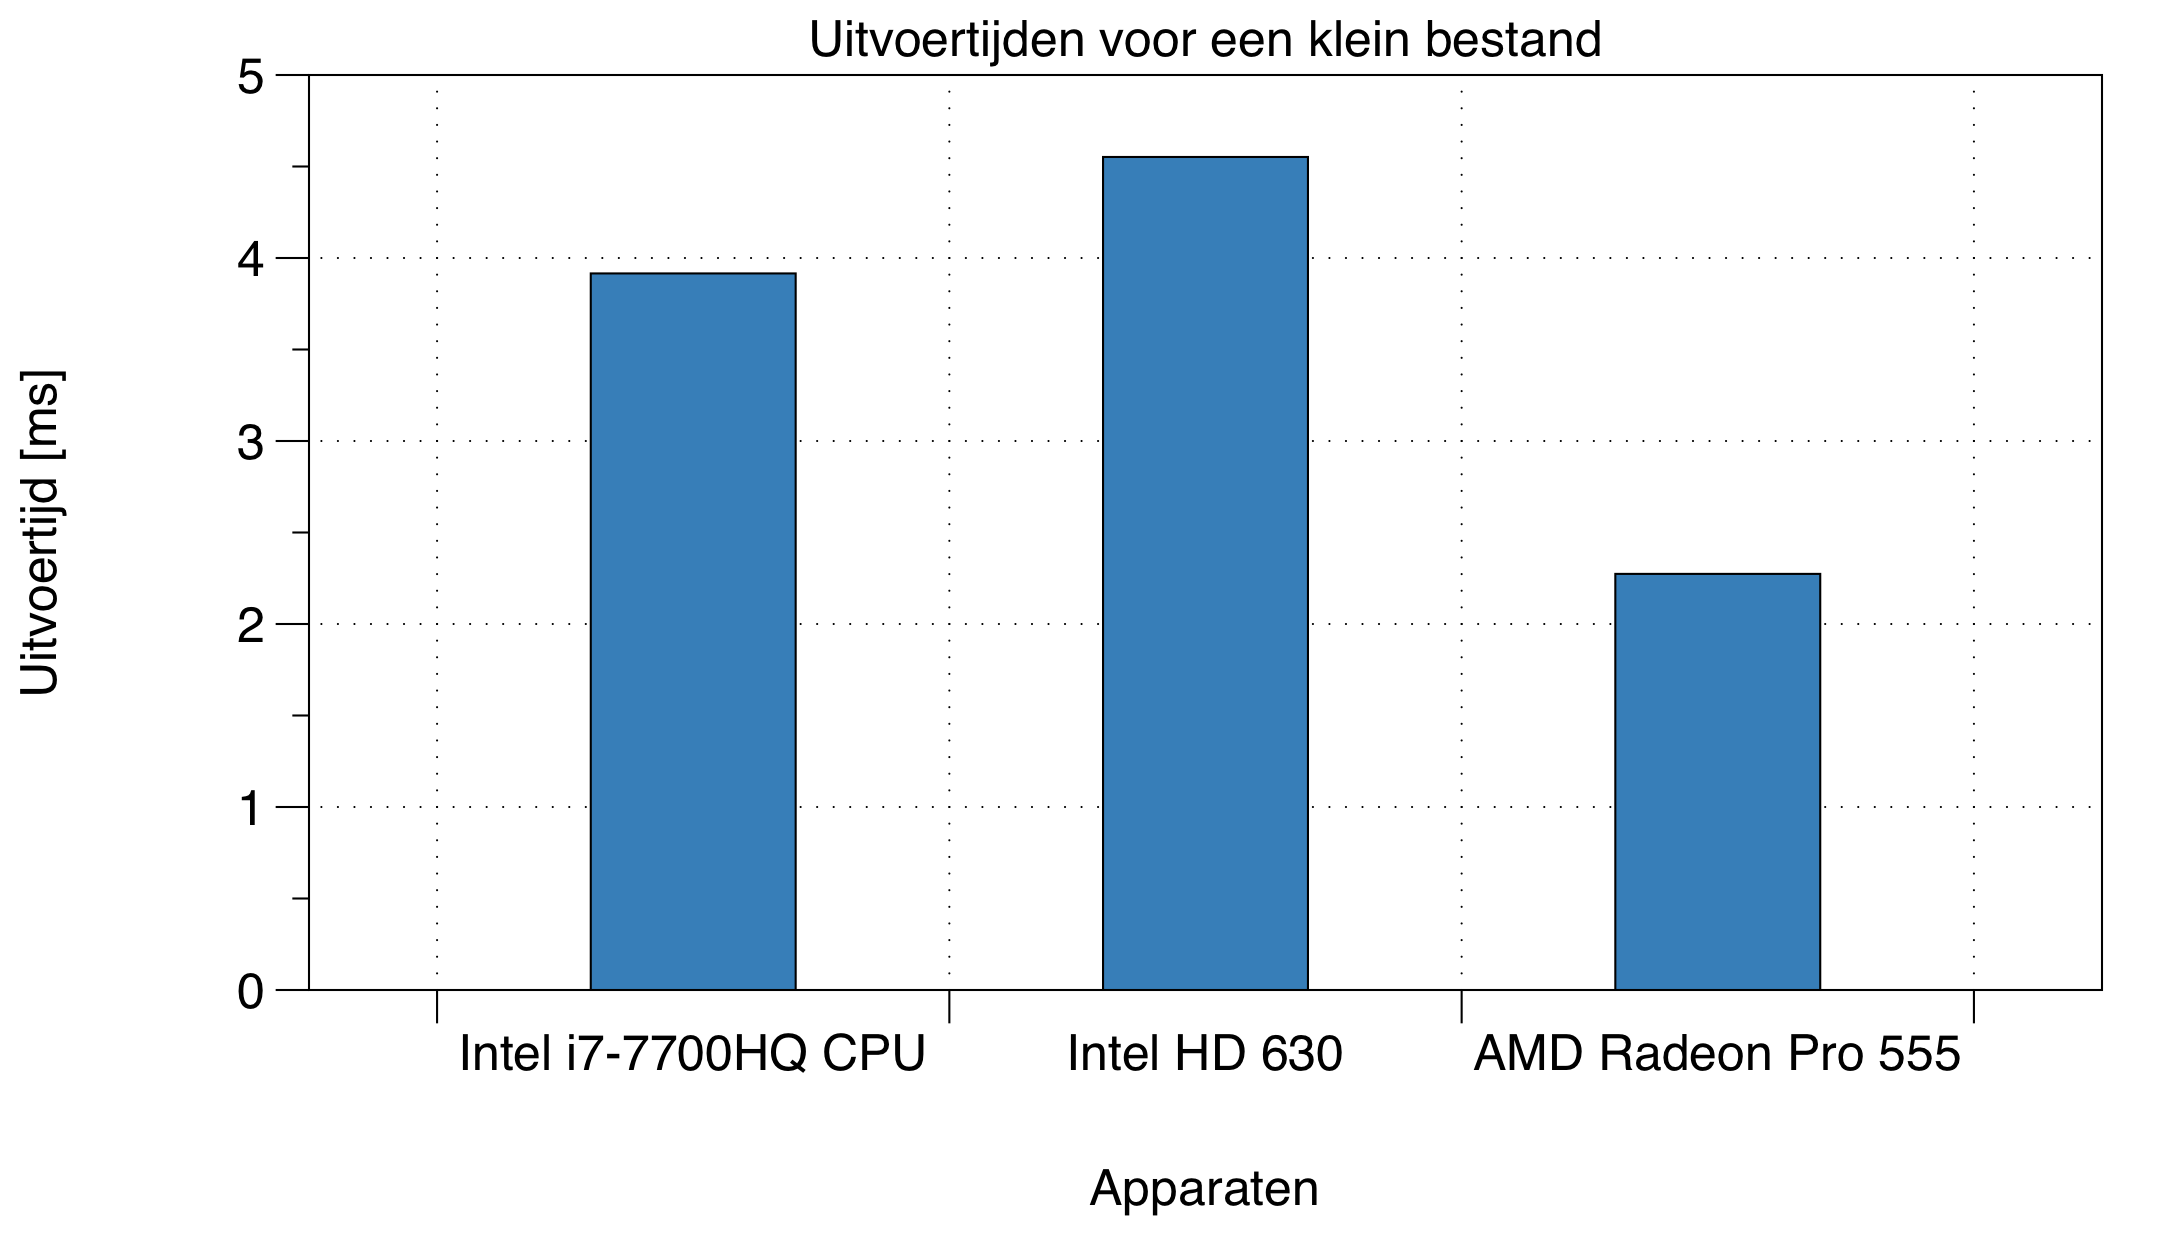
\includegraphics[width=\textwidth]{data/klein.png}
    \end{subfigure}
    \begin{subfigure}{0.5\textwidth}
        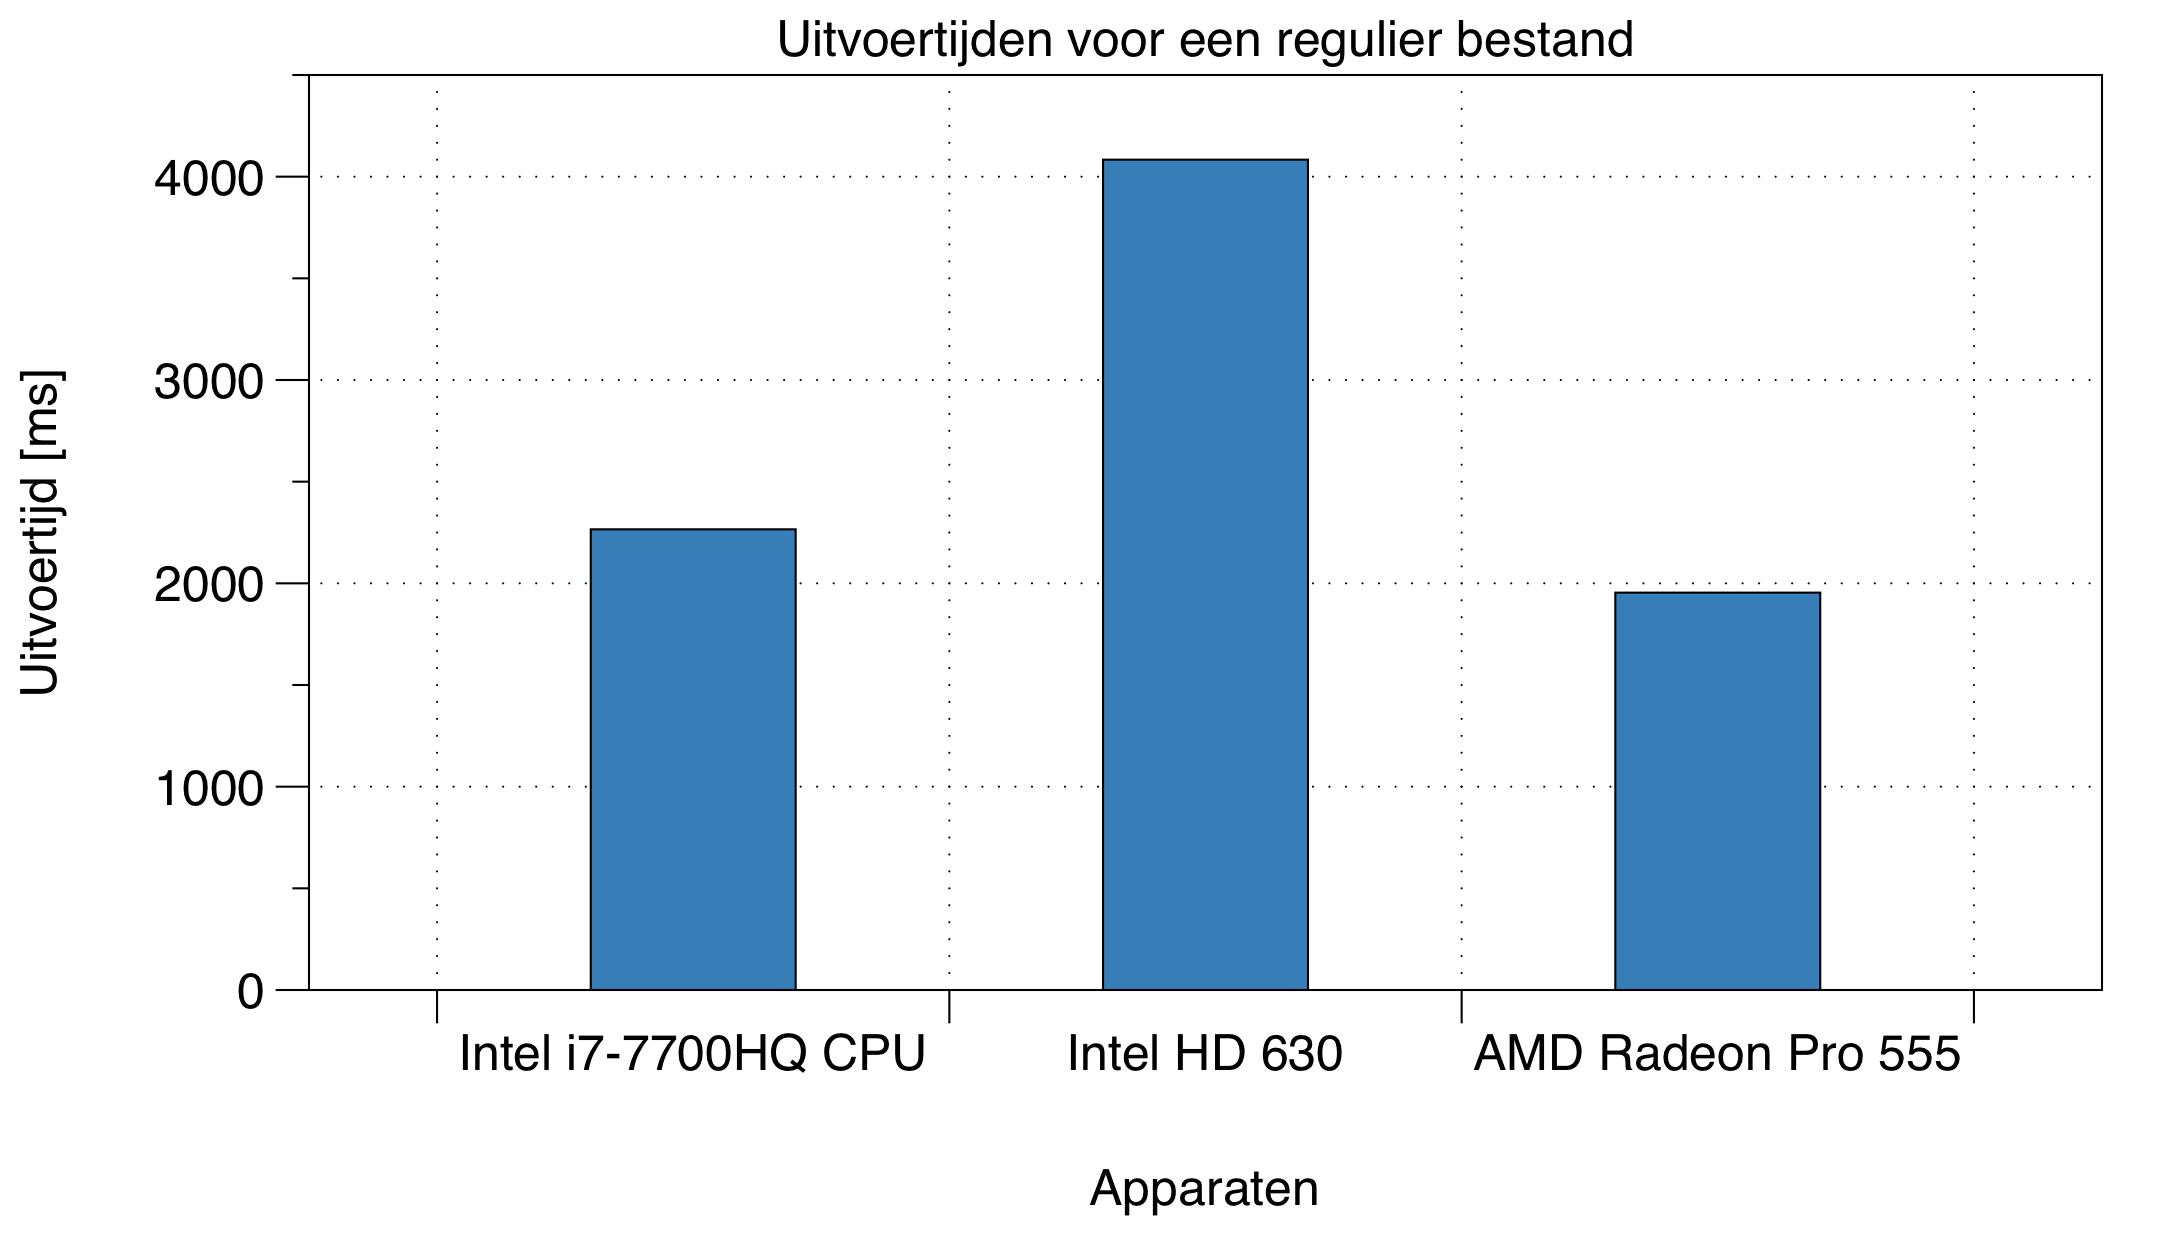
\includegraphics[width=\textwidth]{data/normaal.png}
    \end{subfigure}
    \begin{subfigure}{0.5\textwidth}
        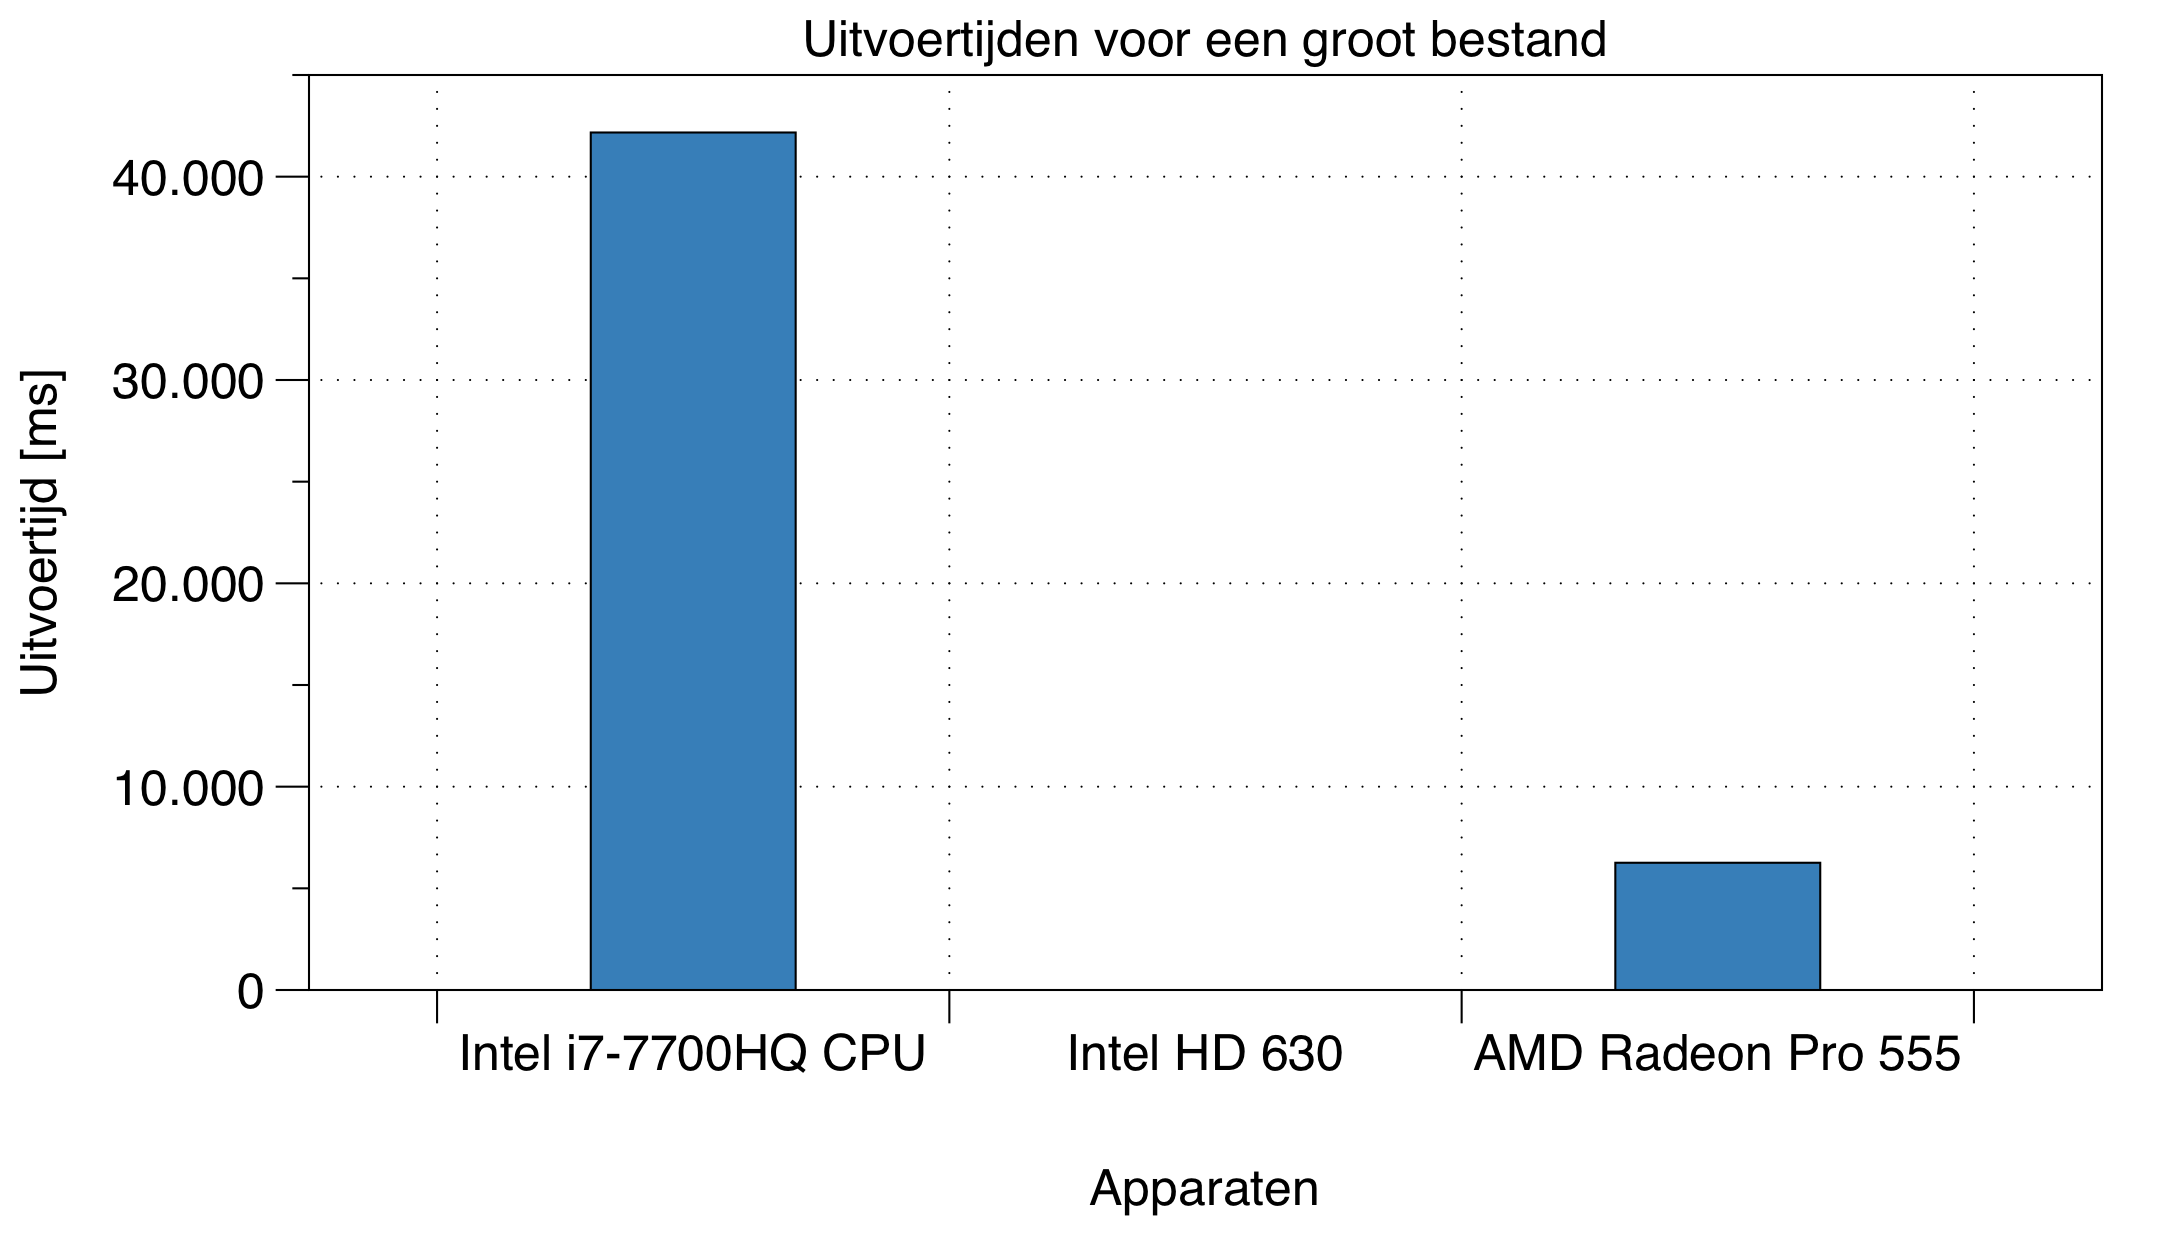
\includegraphics[width=\textwidth]{data/groot.png}
    \end{subfigure}
    \caption{Grafische voorstelling van de data uit Tabel~\ref{table:measurements}.}\label{fig:images}
\end{figure}

\section{Besluit}
Dit verslag werd geschreven als een extra opdracht voor het labo `Geavanceerde computerarchitectuur'. Een pipeline om afbeeldingen te bewerken met behulp van \textit{masks} werd opgezet en ge\"evalueerd.

\onecolumn

\appendix


% Please add the following required packages to your document preamble:
% \usepackage{booktabs}
% \usepackage{longtable}
% Note: It may be necessary to compile the document several times to get a multi-page table to line up properly
\begin{longtable}[c]{@{}rrrrrrrr@{}}
    \caption{My caption}
    \label{my-label}\\
    \toprule
    blocksize & n         & cpu\_swap & cpu\_tot & gpu\_swap   & 2\textasciicircum n & gpu\_tot    & gpu\_delta \\* \midrule
    \endfirsthead
    %
    \multicolumn{8}{c}%
    {{\bfseries Table \thetable\ continued from previous page}} \\
    \toprule
    blocksize & n         & cpu\_swap & cpu\_tot & gpu\_swap   & 2\textasciicircum n & gpu\_tot    & gpu\_delta \\* \midrule
    \endhead
    %
    \bottomrule
    \endfoot
    %
    \endlastfoot
    %
    4         & 1         & 0         & 0        & 0.026720    & 0                   & 0.231104    & 0.204384   \\
    4         & 2         & 0         & 0        & 0.016000    & 1                   & 0.166656    & 0.150656   \\
    4         & 4         & 0         & 0        & 0.015136    & 2                   & 0.157184    & 0.142048   \\
    4         & 8         & 0         & 0        & 0.015136    & 3                   & 0.154304    & 0.139168   \\
    4         & 16        & 0         & 0        & 0.015328    & 4                   & 0.153184    & 0.137856   \\
    4         & 32        & 0         & 0        & 0.015104    & 5                   & 0.152416    & 0.137312   \\
    4         & 64        & 0         & 0        & 0.014528    & 6                   & 0.152352    & 0.137824   \\
    4         & 128       & 0         & 0        & 0.015232    & 7                   & 0.151872    & 0.13664    \\
    4         & 256       & 0         & 0        & 0.015680    & 8                   & 0.153824    & 0.138144   \\
    4         & 512       & 0         & 0        & 0.017248    & 9                   & 0.156480    & 0.139232   \\
    4         & 1024      & 0         & 0        & 0.019648    & 10                  & 0.160800    & 0.141152   \\
    4         & 2048      & 0         & 0        & 0.026048    & 11                  & 0.171136    & 0.145088   \\
    4         & 4096      & 0         & 0        & 0.039392    & 12                  & 0.192640    & 0.153248   \\
    4         & 8192      & 0         & 0        & 0.066496    & 13                  & 0.237408    & 0.170912   \\
    4         & 16384     & 0         & 0        & 0.123200    & 14                  & 0.330976    & 0.207776   \\
    4         & 32768     & 0         & 0        & 0.235488    & 15                  & 0.793952    & 0.558464   \\
    4         & 65536     & 0         & 0        & 0.460480    & 16                  & 5.750496    & 5.290016   \\
    4         & 131072    & 0         & 0        & 0.908800    & 17                  & 1.840640    & 0.93184    \\
    4         & 262144    & 0         & 1        & 1.960640    & 18                  & 3.293632    & 1.332992   \\
    4         & 524288    & 1         & 3        & 3.763616    & 19                  & 5.953568    & 2.189952   \\
    4         & 1048576   & 3         & 6        & 7.537440    & 20                  & 11.550176   & 4.012736   \\
    4         & 2097152   & 6         & 10       & 15.129824   & 21                  & 22.104416   & 6.974592   \\
    4         & 4194304   & 13        & 22       & 30.214945   & 22                  & 43.626751   & 13.411806  \\
    4         & 8388608   & 25        & 42       & 59.756802   & 23                  & 86.269539   & 26.512737  \\
    4         & 16777216  & 51        & 83       & 107.737984  & 24                  & 160.028442  & 52.290458  \\
    4         & 33554432  & 104       & 169      & 192.220093  & 25                  & 297.628571  & 105.408478 \\
    4         & 67108864  & 207       & 337      & 383.706909  & 26                  & 589.636902  & 205.929993 \\
    4         & 134217728 & 411       & 665      & 765.873962  & 27                  & 1176.011108 & 410.137146 \\
    4         & 268435456 & 822       & 1326     & 1532.069702 & 28                  & 2350.672119 & 818.602417 \\
    8         & 1         & 0         & 0        & 0.026720    & 0                   & 0.231104    & 0.204384   \\
    8         & 2         & 0         & 0        & 0.016000    & 1                   & 0.166656    & 0.150656   \\
    8         & 4         & 0         & 0        & 0.015136    & 2                   & 0.157184    & 0.142048   \\
    8         & 8         & 0         & 0        & 0.015136    & 3                   & 0.154304    & 0.139168   \\
    8         & 16        & 0         & 0        & 0.015328    & 4                   & 0.153184    & 0.137856   \\
    8         & 32        & 0         & 0        & 0.015104    & 5                   & 0.152416    & 0.137312   \\
    8         & 64        & 0         & 0        & 0.014528    & 6                   & 0.152352    & 0.137824   \\
    8         & 128       & 0         & 0        & 0.015232    & 7                   & 0.151872    & 0.13664    \\
    8         & 256       & 0         & 0        & 0.015680    & 8                   & 0.153824    & 0.138144   \\
    8         & 512       & 0         & 0        & 0.017248    & 9                   & 0.156480    & 0.139232   \\
    8         & 1024      & 0         & 0        & 0.019648    & 10                  & 0.160800    & 0.141152   \\
    8         & 2048      & 0         & 0        & 0.026048    & 11                  & 0.171136    & 0.145088   \\
    8         & 4096      & 0         & 0        & 0.039392    & 12                  & 0.192640    & 0.153248   \\
    8         & 8192      & 0         & 0        & 0.066496    & 13                  & 0.237408    & 0.170912   \\
    8         & 16384     & 0         & 0        & 0.123200    & 14                  & 0.330976    & 0.207776   \\
    8         & 32768     & 0         & 0        & 0.235488    & 15                  & 0.793952    & 0.558464   \\
    8         & 65536     & 0         & 0        & 0.460480    & 16                  & 5.750496    & 5.290016   \\
    8         & 131072    & 0         & 0        & 0.908800    & 17                  & 1.840640    & 0.93184    \\
    8         & 262144    & 0         & 1        & 1.960640    & 18                  & 3.293632    & 1.332992   \\
    8         & 524288    & 1         & 3        & 3.763616    & 19                  & 5.953568    & 2.189952   \\
    8         & 1048576   & 3         & 6        & 7.537440    & 20                  & 11.550176   & 4.012736   \\
    8         & 2097152   & 6         & 10       & 15.129824   & 21                  & 22.104416   & 6.974592   \\
    8         & 4194304   & 13        & 22       & 30.214945   & 22                  & 43.626751   & 13.411806  \\
    8         & 8388608   & 25        & 42       & 59.756802   & 23                  & 86.269539   & 26.512737  \\
    8         & 16777216  & 51        & 83       & 107.737984  & 24                  & 160.028442  & 52.290458  \\
    8         & 33554432  & 104       & 169      & 192.220093  & 25                  & 297.628571  & 105.408478 \\
    8         & 67108864  & 207       & 337      & 383.706909  & 26                  & 589.636902  & 205.929993 \\
    8         & 134217728 & 411       & 665      & 765.873962  & 27                  & 1176.011108 & 410.137146 \\
    8         & 268435456 & 822       & 1326     & 1532.069702 & 28                  & 2350.672119 & 818.602417 \\
    16        & 1         & 0         & 0        & 0.026112    & 0                   & 0.212128    & 0.186016   \\
    16        & 2         & 0         & 0        & 0.015552    & 1                   & 0.163392    & 0.14784    \\
    16        & 4         & 0         & 0        & 0.014752    & 2                   & 0.154528    & 0.139776   \\
    16        & 8         & 0         & 0        & 0.014464    & 3                   & 0.151776    & 0.137312   \\
    16        & 16        & 0         & 0        & 0.015296    & 4                   & 0.180224    & 0.164928   \\
    16        & 32        & 0         & 0        & 0.014592    & 5                   & 0.158784    & 0.144192   \\
    16        & 64        & 0         & 0        & 0.014400    & 6                   & 0.158816    & 0.144416   \\
    16        & 128       & 0         & 0        & 0.014272    & 7                   & 0.176992    & 0.16272    \\
    16        & 256       & 0         & 0        & 0.014368    & 8                   & 0.147488    & 0.13312    \\
    16        & 512       & 0         & 0        & 0.015232    & 9                   & 0.150240    & 0.135008   \\
    16        & 1024      & 0         & 0        & 0.016448    & 10                  & 0.152800    & 0.136352   \\
    16        & 2048      & 0         & 0        & 0.018784    & 11                  & 0.159200    & 0.140416   \\
    16        & 4096      & 0         & 0        & 0.024192    & 12                  & 0.171392    & 0.1472     \\
    16        & 8192      & 0         & 0        & 0.037280    & 13                  & 0.201152    & 0.163872   \\
    16        & 16384     & 0         & 0        & 0.066144    & 14                  & 0.258336    & 0.192192   \\
    16        & 32768     & 0         & 0        & 0.122656    & 15                  & 0.376064    & 0.253408   \\
    16        & 65536     & 0         & 0        & 0.234016    & 16                  & 0.581184    & 0.347168   \\
    16        & 131072    & 0         & 0        & 0.455616    & 17                  & 1.135360    & 0.679744   \\
    16        & 262144    & 0         & 1        & 0.905600    & 18                  & 1.980800    & 1.0752     \\
    16        & 524288    & 1         & 2        & 1.835616    & 19                  & 3.714080    & 1.878464   \\
    16        & 1048576   & 3         & 5        & 3.770400    & 20                  & 7.434112    & 3.663712   \\
    16        & 2097152   & 6         & 10       & 7.340992    & 21                  & 14.347904   & 7.006912   \\
    16        & 4194304   & 13        & 21       & 15.054016   & 22                  & 28.770657   & 13.716641  \\
    16        & 8388608   & 25        & 41       & 29.408833   & 23                  & 56.575710   & 27.166877  \\
    16        & 16777216  & 52        & 83       & 58.803905   & 24                  & 110.853729  & 52.049824  \\
    16        & 33554432  & 103       & 166      & 117.574974  & 25                  & 221.985474  & 104.4105   \\
    16        & 67108864  & 205       & 332      & 202.782425  & 26                  & 409.763397  & 206.980972 \\
    16        & 134217728 & 410       & 663      & 387.181702  & 27                  & 796.707947  & 409.526245 \\
    16        & 268435456 & 822       & 1327     & 774.899963  & 28                  & 1592.852417 & 817.952454 \\
    32        & 1         & 0         & 0        & 0.026304    & 0                   & 0.222464    & 0.19616    \\
    32        & 2         & 0         & 0        & 0.016640    & 1                   & 0.185024    & 0.168384   \\
    32        & 4         & 0         & 0        & 0.014720    & 2                   & 0.154112    & 0.139392   \\
    32        & 8         & 0         & 0        & 0.014208    & 3                   & 0.181440    & 0.167232   \\
    32        & 16        & 0         & 0        & 0.014336    & 4                   & 0.177856    & 0.16352    \\
    32        & 32        & 0         & 0        & 0.014656    & 5                   & 0.158048    & 0.143392   \\
    32        & 64        & 0         & 0        & 0.014592    & 6                   & 0.158752    & 0.14416    \\
    32        & 128       & 0         & 0        & 0.014688    & 7                   & 0.157952    & 0.143264   \\
    32        & 256       & 0         & 0        & 0.014176    & 8                   & 0.157536    & 0.14336    \\
    32        & 512       & 0         & 0        & 0.023808    & 9                   & 0.180256    & 0.156448   \\
    32        & 1024      & 0         & 0        & 0.014528    & 10                  & 0.161664    & 0.147136   \\
    32        & 2048      & 0         & 0        & 0.015968    & 11                  & 0.166720    & 0.150752   \\
    32        & 4096      & 0         & 0        & 0.017696    & 12                  & 0.182112    & 0.164416   \\
    32        & 8192      & 0         & 0        & 0.022496    & 13                  & 0.187392    & 0.164896   \\
    32        & 16384     & 0         & 0        & 0.037312    & 14                  & 0.231520    & 0.194208   \\
    32        & 32768     & 0         & 0        & 0.066176    & 15                  & 0.350176    & 0.284      \\
    32        & 65536     & 0         & 0        & 0.122432    & 16                  & 0.471936    & 0.349504   \\
    32        & 131072    & 0         & 0        & 0.233632    & 17                  & 0.789696    & 0.556064   \\
    32        & 262144    & 0         & 1        & 0.458528    & 18                  & 1.472128    & 1.0136     \\
    32        & 524288    & 1         & 2        & 0.924256    & 19                  & 2.858368    & 1.934112   \\
    32        & 1048576   & 3         & 5        & 1.948992    & 20                  & 5.999584    & 4.050592   \\
    32        & 2097152   & 6         & 10       & 3.675776    & 21                  & 10.638464   & 6.962688   \\
    32        & 4194304   & 12        & 21       & 8.781536    & 22                  & 22.679840   & 13.898304  \\
    32        & 8388608   & 25        & 42       & 16.280865   & 23                  & 43.810944   & 27.530079  \\
    32        & 16777216  & 52        & 84       & 29.393312   & 24                  & 82.480515   & 53.087203  \\
    32        & 33554432  & 104       & 168      & 59.686562   & 25                  & 164.604218  & 104.917656 \\
    32        & 67108864  & 207       & 333      & 107.966850  & 26                  & 313.733124  & 205.766274 \\
    32        & 134217728 & 413       & 665      & 193.956741  & 27                  & 604.857605  & 410.900864 \\
    32        & 268435456 & 823       & 1329     & 386.880005  & 28                  & 1209.285767 & 822.405762 \\
    48        & 1         & 0         & 0        & 0.024352    & 0                   & 0.203904    & 0.179552   \\
    48        & 2         & 0         & 0        & 0.015008    & 1                   & 0.168512    & 0.153504   \\
    48        & 4         & 0         & 0        & 0.014016    & 2                   & 0.162432    & 0.148416   \\
    48        & 8         & 0         & 0        & 0.014208    & 3                   & 0.160384    & 0.146176   \\
    48        & 16        & 0         & 0        & 0.014112    & 4                   & 0.236672    & 0.22256    \\
    48        & 32        & 0         & 0        & 0.014560    & 5                   & 0.162560    & 0.148      \\
    48        & 64        & 0         & 0        & 0.014112    & 6                   & 0.160960    & 0.146848   \\
    48        & 128       & 0         & 0        & 0.014624    & 7                   & 0.187328    & 0.172704   \\
    48        & 256       & 0         & 0        & 0.014656    & 8                   & 0.164448    & 0.149792   \\
    48        & 512       & 0         & 0        & 0.014976    & 9                   & 0.160960    & 0.145984   \\
    48        & 1024      & 0         & 0        & 0.014848    & 10                  & 0.162624    & 0.147776   \\
    48        & 2048      & 0         & 0        & 0.015232    & 11                  & 0.167040    & 0.151808   \\
    48        & 4096      & 0         & 0        & 0.016096    & 12                  & 0.175808    & 0.159712   \\
    48        & 8192      & 0         & 0        & 0.016160    & 13                  & 0.182944    & 0.166784   \\
    48        & 16384     & 0         & 0        & 0.022400    & 14                  & 0.216576    & 0.194176   \\
    48        & 32768     & 0         & 0        & 0.037568    & 15                  & 0.280800    & 0.243232   \\
    48        & 65536     & 0         & 0        & 0.067936    & 16                  & 0.238176    & 0.17024    \\
    48        & 131072    & 0         & 0        & 0.123136    & 17                  & 0.680448    & 0.557312   \\
    48        & 262144    & 0         & 1        & 0.236832    & 18                  & 1.290016    & 1.053184   \\
    48        & 524288    & 1         & 2        & 0.470592    & 19                  & 2.380192    & 1.9096     \\
    48        & 1048576   & 3         & 5        & 0.933216    & 20                  & 4.728096    & 3.79488    \\
    48        & 2097152   & 6         & 10       & 1.853792    & 21                  & 8.841728    & 6.987936   \\
    48        & 4194304   & 13        & 22       & 3.697664    & 22                  & 17.433249   & 13.735585  \\
    48        & 8388608   & 25        & 42       & 8.022368    & 23                  & 35.602783   & 27.580415  \\
    48        & 16777216  & 53        & 84       & 14.867776   & 24                  & 68.187134   & 53.319358  \\
    48        & 33554432  & 103       & 166      & 29.551424   & 25                  & 132.463577  & 102.912153 \\
    48        & 67108864  & 205       & 331      & 59.075008   & 26                  & 264.489380  & 205.414372 \\
    48        & 134217728 & 410       & 663      & 101.647873  & 27                  & 511.711060  & 410.063187 \\
    48        & 268435456 & 821       & 1325     & 195.260696  & 28                  & 1012.969238 & 817.708542 \\
    64        & 1         & 0         & 0        & 0.030528    & 0                   & 0.271072    & 0.240544   \\
    64        & 2         & 0         & 0        & 0.157792    & 1                   & 0.325760    & 0.167968   \\
    64        & 4         & 0         & 0        & 0.014368    & 2                   & 0.164512    & 0.150144   \\
    64        & 8         & 0         & 0        & 0.016064    & 3                   & 0.189952    & 0.173888   \\
    64        & 16        & 0         & 0        & 0.014048    & 4                   & 0.564256    & 0.550208   \\
    64        & 32        & 0         & 0        & 0.016672    & 5                   & 0.169472    & 0.1528     \\
    64        & 64        & 0         & 0        & 0.015424    & 6                   & 0.155520    & 0.140096   \\
    64        & 128       & 0         & 0        & 0.015296    & 7                   & 0.150720    & 0.135424   \\
    64        & 256       & 0         & 0        & 0.014816    & 8                   & 0.149440    & 0.134624   \\
    64        & 512       & 0         & 0        & 0.014048    & 9                   & 0.150624    & 0.136576   \\
    64        & 1024      & 0         & 0        & 0.014336    & 10                  & 0.151456    & 0.13712    \\
    64        & 2048      & 0         & 0        & 0.014976    & 11                  & 0.155552    & 0.140576   \\
    64        & 4096      & 0         & 0        & 0.016608    & 12                  & 0.164320    & 0.147712   \\
    64        & 8192      & 0         & 0        & 0.018880    & 13                  & 0.183712    & 0.164832   \\
    64        & 16384     & 0         & 0        & 0.027776    & 14                  & 0.221888    & 0.194112   \\
    64        & 32768     & 0         & 0        & 0.047616    & 15                  & 0.303904    & 0.256288   \\
    64        & 65536     & 0         & 0        & 0.084352    & 16                  & 0.433792    & 0.34944    \\
    64        & 131072    & 0         & 0        & 0.158464    & 17                  & 0.710656    & 0.552192   \\
    64        & 262144    & 0         & 1        & 0.308576    & 18                  & 1.361824    & 1.053248   \\
    64        & 524288    & 1         & 2        & 0.611680    & 19                  & 2.511168    & 1.899488   \\
    64        & 1048576   & 3         & 5        & 1.213408    & 20                  & 4.807776    & 3.594368   \\
    64        & 2097152   & 6         & 10       & 2.416928    & 21                  & 9.344544    & 6.927616   \\
    64        & 4194304   & 12        & 21       & 6.361856    & 22                  & 19.720287   & 13.358431  \\
    64        & 8388608   & 25        & 41       & 10.310720   & 23                  & 36.748512   & 26.437792  \\
    64        & 16777216  & 51        & 82       & 19.302591   & 24                  & 71.741600   & 52.439009  \\
    64        & 33554432  & 104       & 168      & 38.599712   & 25                  & 143.883652  & 105.28394  \\
    64        & 67108864  & 207       & 335      & 70.304253   & 26                  & 277.131866  & 206.827613 \\
    64        & 134217728 & 412       & 665      & 131.725540  & 27                  & 541.917847  & 410.192307 \\
    64        & 268435456 & 832       & 1344     & 253.048996  & 28                  & 1070.998413 & 817.949417 \\
    128       & 2         & 0         & 0        & 0.017248    & 1                   & 0.207552    & 0.190304   \\
    128       & 4         & 0         & 0        & 0.016160    & 2                   & 0.199040    & 0.18288    \\
    128       & 8         & 0         & 0        & 0.016160    & 3                   & 0.195264    & 0.179104   \\
    128       & 16        & 0         & 0        & 0.016000    & 4                   & 0.193728    & 0.177728   \\
    128       & 32        & 0         & 0        & 0.016512    & 5                   & 0.194656    & 0.178144   \\
    128       & 64        & 0         & 0        & 0.015776    & 6                   & 0.195552    & 0.179776   \\
    128       & 128       & 0         & 0        & 0.016768    & 7                   & 0.194880    & 0.178112   \\
    128       & 256       & 0         & 0        & 0.016288    & 8                   & 0.195200    & 0.178912   \\
    128       & 512       & 0         & 0        & 0.016256    & 9                   & 0.197152    & 0.180896   \\
    128       & 1024      & 0         & 0        & 0.015904    & 10                  & 0.199072    & 0.183168   \\
    128       & 2048      & 0         & 0        & 0.017600    & 11                  & 0.204096    & 0.186496   \\
    128       & 4096      & 0         & 0        & 0.018336    & 12                  & 0.214816    & 0.19648    \\
    128       & 8192      & 0         & 0        & 0.019488    & 13                  & 0.239008    & 0.21952    \\
    128       & 16384     & 0         & 0        & 0.022496    & 14                  & 0.230880    & 0.208384   \\
    128       & 32768     & 0         & 0        & 0.037728    & 15                  & 0.297472    & 0.259744   \\
    128       & 65536     & 0         & 0        & 0.065792    & 16                  & 0.437600    & 0.371808   \\
    128       & 131072    & 0         & 0        & 0.122912    & 17                  & 0.674944    & 0.552032   \\
    128       & 262144    & 0         & 1        & 0.238368    & 18                  & 1.302016    & 1.063648   \\
    128       & 524288    & 1         & 2        & 0.466976    & 19                  & 2.568128    & 2.101152   \\
    128       & 1048576   & 3         & 5        & 0.915232    & 20                  & 4.718944    & 3.803712   \\
    128       & 2097152   & 6         & 11       & 1.818912    & 21                  & 8.777664    & 6.958752   \\
    128       & 4194304   & 12        & 21       & 5.163584    & 22                  & 18.596512   & 13.432928  \\
    128       & 8388608   & 26        & 41       & 7.805344    & 23                  & 34.176674   & 26.37133   \\
    128       & 16777216  & 51        & 83       & 14.505632   & 24                  & 67.594078   & 53.088446  \\
    128       & 33554432  & 103       & 166      & 28.994144   & 25                  & 131.901794  & 102.90765  \\
    128       & 67108864  & 205       & 333      & 58.011265   & 26                  & 263.177185  & 205.16592  \\
    128       & 134217728 & 410       & 663      & 97.118210   & 27                  & 506.298584  & 409.180374 \\
    128       & 268435456 & 821       & 1324     & 190.015869  & 28                  & 1008.206482 & 818.190613 \\* \bottomrule
    \end{longtable}

\newpage

% The appendix command is issued once, prior to all appendices, if any.
%\appendix
\end{document}

